% To check in final format
%\documentclass[final,twocolumn]{elsarticle}
\documentclass[preprint,review,12pt]{elsarticle}


\usepackage{amssymb}
\usepackage{graphicx}
\usepackage{multirow}
\usepackage{tabularx}
\usepackage{booktabs}
\usepackage[noend]{algpseudocode}
\usepackage{subfig}
\usepackage[table,xcdraw]{xcolor}
\usepackage{amsthm}
\usepackage{color}
\usepackage{soul}
\usepackage{ulem}
\usepackage{amsmath}
\usepackage{float}

\newcommand{\hlr}[2][red]{
  {\sethlcolor{#1} \hl{#2}}
}

\newcommand{\hly}[2][yellow]{
  {\sethlcolor{#1} \hl{#2}}
}
\newcommand{\hlg}[2][green]{
  {\sethlcolor{#1} \hl{#2}}
}
\newcommand{\hlp}[2][pink]{
  {\sethlcolor{#1} \hl{#2}}
}

\usepackage{lineno,hyperref}
\modulolinenumbers[5]

\journal{Journal of \LaTeX\ Templates}

\bibliographystyle{elsarticle-num}

\begin{document}

\begin{frontmatter}

\title{Joint Service Chain Deployment and Manager Placement in NFV}

\author[aut]{Parham Alvani}
\ead{parham.alvani@aut.ac.ir}

\author[aut]{Bahador Bakhshi
\corref{correspondingauthor}}
\ead{bbakhshi@aut.ac.ir}

\cortext[correspondingauthor]{Corresponding author.}

\address[aut]{Amirkabir University of Technology, Tehran, Iran}

\begin{abstract}
\hly{%
a) Motivation \\
b) Introduce the problem \\
c) Why is there a research gap \\
d) What have we done \\
e) What are the results \\
}
In the old times, Network providers use physical network functions to create their service chains, but a single change in this manner is difficult and may cause many service disruption.
SFC and NFV is the solution to this difficulty. By using SFC and NFV, providers can provision chains dynamically and then change them in the run-time.
One of the main requirements this virtualized environment is management and monitoring for the chains.
In this research, we consider the chain acceptance problem subject to management resources. In the first step, we formulate
problem with ILP and then implement it in CPLEX framework. The optimal solution takes time to solve so we need a Polynomial-Time solution to the problem.
In this research, we develop a heuristic algorithm and compare its result with the optimal solution. In the end, the heuristic solution produces near-optimal results in the polynomial time.
\end{abstract}

\begin{keyword}
\end{keyword}

\end{frontmatter}

\section{Introduction}
\hly{%
a) A general introduction of the context \\
b) More specific context of problem and its importance \\
c) A very brief review of literature and introduce the research gap \\
d) What is the problem \\
e) What are the contributions \\
f) The structure of the paper \\
}
In NFV ecosystem, each chain must be monitored and managed by a VNFM. Similar to other virtual functions, VNFMs need computing and network resources and  can manage a limited number of chains.
Our work considers Service Chain Placement Problem and Manager Placement Problem jointly and wants to place chains and their corresponding VNFM at the same time.
We believe this work hasn't been done in the literature before.
By considering the joint problem, you may not accept a chain that you don't have any management resource for it,
or you can get many chains that have little management resource requirement.
These considerations create a better solution with more profit to datacenter from provisioning the set of chains,
and the results in \ref{sec:joint-vs-disjoint} approves it.



\section{Related Work}\label{sec:related-works}
In this section, we review the works that have been done on service chain deployment and resource assignment in NFV, and mainly we focus on the works that consider management requirements of chains.

In NFV, resource assignment is composed of
allocating computing and memory resources for virtual machines to run the chains' virtual network functions and assigning network resources to the chains' virtual links. Various objective functions, e.g., minimizing cost, maximizing profit and minimizing power consumption can be aimed in the resource management problem where a wide range of additional, e.g., end-to-end delay, fault tolerance as well as management requirements need to be satisfied.

\subsection{Resource Allocation in NFV}
The VNF placement problem has received substantial attention in the literature \cite{GilHerrera2016}.
We will concentrate on network function chain placement which dynamically steers
traffic through an ordered list of Service Functions from 3 categories that are discussed in \cite{Laghrissi2019}.
Objectives like energy consumption minization, cost optimization, Quality of Service (QoS), resource usage, reliablity,
and load balancing.

\subsection{Management Resources in NFV}
As already mentioned, this work considers management resources. To best of our knowledge, work \cite{AbuLebdeh2017}, its next work \cite{AbuLebdeh20172}, and \cite{Chiang2019} are the only ones that consider VNFM and other management resources in SFC deployment.

In \cite{AbuLebdeh2017}, the authors studied the problem of VNFM placement in a distributed NFV infrastructure under the assumption that chains have already been deployed and consequently, the location of VNFs are known.
The objective function of the VNFM placement problem is to minimize the operational costs which is:
\begin{itemize}
    \item Life cycle Management Cost
    \item Compute Resources Cost
    \item Migration Cost
    \item Reassignment Cost
\end{itemize}
Delay constraint on management links is also considered.
The authors used tabu search algorithm because of its superior results to other techniques in FLP, for finding a polynomial solution. They start from a feasible placement and each step they improve VNFM placement by doing one of these moves:
\begin{itemize}
    \item Reassignment
    \item Relocation
    \item Bulk
    \item Deactivation
\end{itemize}
While this is the first work that investigated the management resource assignment in NFV, it does not the joint SFC deployment and VNFM placement.

In \cite{AbuLebdeh20172} authors solve VNFO placement problem that is far from our current work that doesn't consider VNFO.
Authors consider the same system as \cite{AbuLebdeh2017} but here they want to place VNFO and VNFM jointly, trying to minimize operational cost as defined by \cite{AbuLebdeh2017}.
They propose a two step placement algorithm that first place VNFOs and then place VNFMs. Each of these steps use Tabu-Search method.

In \cite{Chiang2019} authors consider autonomy for VNFMs that selects their managed VNFs dynamically and use game theory to achieve a distributed solution to the VNFM Placement Problem as desribed in \cite{AbuLebdeh2017}.
Authors consider the same system model from \cite{AbuLebdeh2017} and try minimize operational cost consists of bandwidth cost and compute cost.
In our work relation between VNFMs and VNFs are static and VNFM cannot change these relation by their own.

To conclude, the problem of joint SFC deployment and VNFMs placement has not yet been consider. In the rest of this paper, we formulate the problem and propose solution for it.

\subsection{Current Work}

Our work considers the above problems jointly and wants to place chains and their corresponding VNFM at the same time.
We believe this work hasn't been done in the literature before.
By considering the joint problem, you may not accept a chain that you don't have any management resource for it,
or you can get many chains that have little management resource requirement.
These considerations create a better solution with more profit to datacenter from provisioning the set of chains,
and the results in \ref{sec:joint-vs-disjoint} approves it.
The closest work to current research is \cite{AbuLebdeh2017} but it assumes that the VNFs' placement is known and solves only the VNF manager placement problem. Current research also considers more constraints that \cite{AbuLebdeh2017} on VNFM placements that we discuss deeply in the following sections and summarize them here:

\begin{itemize}
    \item Current research considers license cost for VNFM instances
    \item In current research each physical node has its specific list of nodes that can run its VNFM. This constraint provides a great flexibility for implementing management policies.
\end{itemize}

At the end current research and \cite{AbuLebdeh2017} have different objectives but we will try to compare their results and solutions.


\section{System Model and Problem Statement}\label{sec:system-model}
In this section, after discussing the assumptions and system model, the problem of joint SFC deployment and VNFM placement is stated and clarified by an illustrative example.

\subsection{Assumptions}\label{subsec:assumptions}
In the JSD-MP problem, a set of SFCs need to be deployed in the physical infrastructure network.
The main assumption is that in addition to computational and network resources,
a VNFM should be assigned for each SFC to manage the VNFs of the SFC.
All VNFs of a chain should be managed by a single VNFM, but a VNFM can manage multiple SFCs.
The capacity of each VNFM is limited in terms of the number of VNF instances.
Each VNFM needs a license for managing the specific number of VNF instances.
Moreover, we assume that only a subset of physical servers can host VNFMs and similarly,
each VNF type can only be placed on a subset of physical servers. It is assumed that traffic ingress and egress of each chain are conducted by a special type of NFVs, which need to be placed on ingress and egress nodes  of the physical network respectively.

VNF instances deployed on a physical server can only be managed by the VNFMs placed on a given subset of physical servers. To maintain the timing requirement of the management traffic, the distance (in term of hop-count) between each VNFM and its associated VNFs should be less than the specified threshold.
Also, JSD-MP considers VNFs can't shared between chains.
% Only a subset of VNF types need to managed and other can be deployed without an assigned VNFM.

\subsection{System Model}\label{subsec:sysmodel}
% parameters will define here and decision variables will defined in formulation section.
%
%% Infrastructure's parameters have superscript "p"
%% Chain's parameters have superscript "s"
%% Infrastructure's nodes have subscript "i", "j"
%% Chain's nodes have subscript "u", "v"
%% Use parentheses for functions and in rare occasions
%% Management's parameters have superscript "m"
%% Use capital letters for sets
%

The physical infrastructure topology is modeled as a directed graph \(G^p=(V^p, E^p)\),
where \(V^p\) is the set of NFVI-PoPs and \(E^p\) is a set of the inter-PoP links.
The computational capacity of PoP \(i \in V^p\) is specified by \(c^p_i\) number of CPU cores and \(m^p_i\) gigabytes of RAM.
Bandwidth of link \((i,j) \in E^p\) is specified by \(b^p_{(i.j)}\).

The set of requested SFCs is denoted by \(R\).
Each request \(r \in R\) has revenue \(c_r\) and
is represented by directed graph \(G^s_r = (V^s_r, E^s_r)\),
where \(V^s_r\) is the set of VNFs and \(E^s_r\) is the set of the virtual links of the chain.
The type of VNF \(v \in V^s_r\) is denoted by \(t_{v,r} \in T\) where \(T\) is the set of the types of the functions.
Each type \(t\) determines the required number of CPU cores \(c^s_t\)
and the required amount of memory \(m^s_t\) to create an instance of that type.
The required bandwidth of each virtual link \((u,v) \in E^s_r\) is denoted by \(b^s_{(u,v),r}\).

Each VNFM requires \(c^m\) number of CPU cores and \(m^m\) gigabytes of RAM to handle \(\kappa\) number of VNFs at most. To lunching a VNFM, the service provider has to pay the license fee \(\phi\).
There is a dedicated virtual management link with bandwidth \(b^m\) between every VNF instance and its associated VNFM.
The restrictions of the placement of VNFMs and VNFs, discussed in the previous section, are formulated by a few given parameters.
We use \(\rho\) to indicate the maximum hop counts for each virtual management link. Parameter \(\eta_{(i, j)}\) indicates whether the VNFM mapped to the physical server \(i \in V^p\) can manage the VNFs placed on the physical node \(j \in V^p\) or not. 
% Parameter \(\omega_r\) indicates that type \(r \in T\) requires manager or not.
% The binary parameter \(\psi_i\) indicates that physical server \(i \in V^p\) support VNFs or not.
The notations discussed here are summarized in Table \ref{tbl:parameters}.

\begin{table}
    \caption{Parameters}
    \label{tbl:parameters}
    \begin{small}
    \begin{center}\begin{tabular}{|c|p{0.75\textwidth}|}
    \hline
    \(V^p\) & the set of NFVI-PoPs \\
    \hline
    \(E^p\) & the set of the inter-PoP links \\
    \hline
    \(c^p_i\) & number of CPU cores of server \(i\) \\
    \hline
    \(m^p_i\) & amount of RAM in server \(i\) \\
    \hline
    \(b^p_(i,j)\) & bandwidth of link \((i, j) \in E^p \) \\
    \hline
    \(V^s_r\) & the set of VNFs for the request \(r\) \\
    \hline
    \(E^s_r\) & the set of virtual links of the request \(r\) \\
    \hline
    \(m^s_t\) & required RAM of VNF instance with type \(t \in T\) in GB \\
    \hline
    \(c^s_t\) & required CPU cores of VNF instance with type \(t \in T\) \\
    \hline
    \(m^m\) & required RAM of VNFM in GB \\
    \hline
    \(c^m\) & required CPU cores of VNFM \\
    \hline
    \(\kappa\) & maximum number of VNF instances that a VNFM can handle \\
    \hline
    \(\tau(v, t)\) & function that returns 1 if the VNF instance \(v\) has type \(t\)  \\
    \hline
    \(b^s_{(u, v),r}\) & required bandwidth for virtual link \((u, v) \in E^s_r\) \\
    \hline
    \(b^m\) & required bandwidth for each virtual management link \\
    \hline
    \(\rho\) & maximum hop count of management links \\
    \hline
    \(\phi\) & VNFM license fee \\
    \hline
    \(\eta_{(i, j)}\) & binary parameter that is 1 if VNFs on physical server \(i\) can manage by VNFMs on physical server \(j\) \\
    \hline
    \end{tabular}\end{center}
    \end{small}
\end{table}

\subsection{Problem Statement}
Under the assumptions of subsection \ref{subsec:assumptions}, the JSD-MP problem is defined as following using the notations defined in subsection \ref{subsec:sysmodel}.
The NFVI service provider owns the infrastructure network \(G^p\). A set \(R\) of requests are given. The service provider's goal is to accept a subset of requests that maximize the profit.
To accept a request \(r\), the service provider should allocate the \(c^s_{t_{v,r}}\) CPU cores, and \(m^s_{t_{v,r}}\) amount of memory for all \(v \in r\);
moreover, \(b^s_{(u,v),r}\) bandwidth should be allocated for all links \((u,v) \in E^s_r\), and a VNFM needs to be assigned for the chain.
These allocations should satisfy the requirements mentioned in subsection \ref{subsec:assumptions}.
The profit is made by the revenue obtained from accepting the requests while the service provider should pay the license cost of \(\phi\) for each VNFM.

The idea behind the JSD-MP problem is that in the placement of VNFM for a chain, the location of the VNFs of the chain should be taken into account. Therefore, by jointly conducting of SFC deployment and VNFM placement, the service provider can maximize the profit.

This problem is clarified by an illustrative example in the following subsection.

\subsection{Illustrative Example}
In this section, an illustrative example is presented to gain more sight into the JSD-MP problem.
Figure~\ref{fig:example-chains} shows two request chains where the type of VNFs and the required bandwidth of the virtual links in Mbps are depicted. Each of these requests worth 100\$.
The NFVI service provider owns the infrastructure that is shown in Figure~\ref{fig:example-topology}.
VNF's types are described in Table~\ref{tbl:example-vnf-types}, and 
Table~\ref{tbl:example-server-spec} shows the physical servers specifications.
There a few constraints on placing the VNFs and capacity of the NFVI as following.
Instances can only run on servers 1, 3, 5, and 7 since the remaining servers are fully utilized.
The VNFs on servers 1 and 3 can only be managed by the VNFMs on servers 2 and 4.
The VNFs on server 5 can only be managed by the VNFMs on servers 4 and 6.
The VNFs on server 7 can only be managed by the VNFMs on servers 6 and 8.
Each VNFM can handles at most 5 instances with 4 GB of RAM and 2 CPU cores and license that costs 10\$.
Management links requires 10Mbps reservation and maximum hop counts for management is 10.
All physical links has 40Gbps capacity. 

\begin{figure}
    \centering
    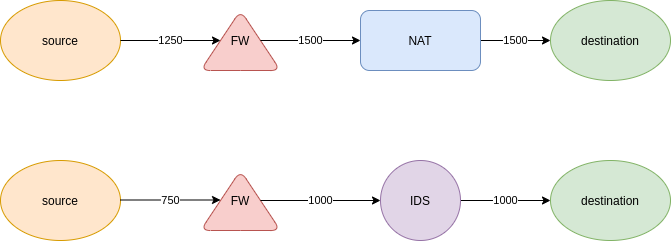
\includegraphics[width=0.7\linewidth]{images/example-chains.png}
    \caption{Chains for illustrative example}
    \label{fig:example-chains}
\end{figure}

\begin{figure}
    \centering
    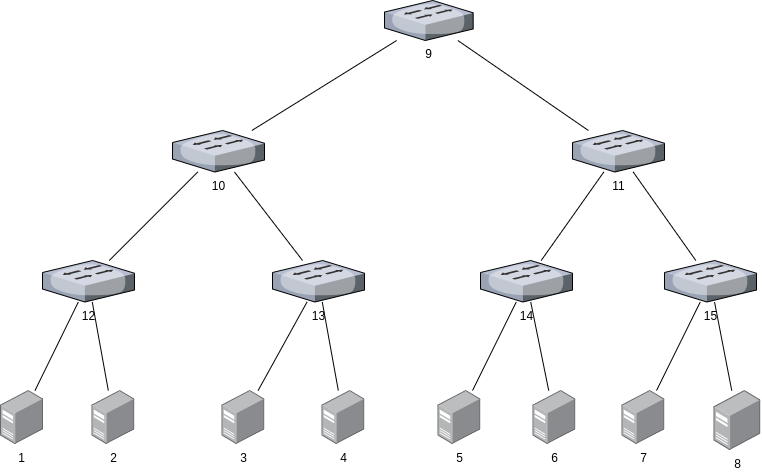
\includegraphics[height=150px]{images/example-toplogy.png}
    \caption{Topology of illustrative example}
    \label{fig:example-topology}
\end{figure}

\begin{table}
    \centering
    \caption{VNFs type of illustrative example}
    \begin{tabular}{|c|c|c|c|}
        \hline
        Spec/VNF & vFW & vNAT & vIDS \\
        \hline
        CPU (vCore) & 2 & 2 & 2 \\
        \hline
        Memory (GB) & 2 & 4 & 2 \\
        \hline
    \end{tabular}
    \label{tbl:example-vnf-types}
\end{table}

\begin{table}
    \centering
    \caption{Server specification of illustrative example}
    \begin{tabular}{|c|c|c|}
        \hline
        & Server 1,2,7,8 & Servers 3,4,5,6 \\
        \hline
        Installed vCPU & 144 & 72 \\
        \hline
        Installed Memory (GB) & 1408 & 288 \\
        \hline
        Link (Gbps) & 40 & 40 \\
        \hline
    \end{tabular}
    \label{tbl:example-server-spec}
\end{table}

The optimal solution of this instance of the JSD-MP, which is obtained by the MILP formulation presented in section~\ref{sec:formulation}, is as following:

Two chains are accepted with using two VNFM instances that cost 20 so the total revenue is 180.
Instance mappings are shown in \ref{tbl:example-chain-1-mapping} and \ref{tbl:example-chain-2-mapping}.
Also link mappings are shown in \ref{tbl:example-chain-1-links}.

\begin{table}
    \centering
    \caption{Chain-1 Instance Mapping of illustrative example}
    \begin{tabular}{|c|c|c|c|c|}
        \hline
        0: Source & 1: FW & 2: NAT & 3: Destination & VNFM \\
        \hline
        9 & 1 & 3 & 9 & 4 \\
        \hline
    \end{tabular}
    \label{tbl:example-chain-1-mapping}
\end{table}

\begin{table}
    \centering
    \caption{Chain-1 Instance Mapping of illustrative example}
    \begin{tabular}{|c|c|c|c|c|}
        \hline
        0: Source & 1: FW & 2: IDS & 3: Destination & VNFM \\
        \hline
        9 & 3 & 3 & 9 & 4 \\
        \hline
    \end{tabular}
    \label{tbl:example-chain-2-mapping}
\end{table}

\begin{table}
    \centering
    \caption{Chain-1 Link Mapping of illustrative example}
    \begin{tabular}{|c|l|}
        \hline
        Virtual Link & Physical Links \\
        \hline
        (0, 1) & (9, 10) (10, 12) (12, 1) \\
        \hline
        (1, 2) & (1, 12) (12, 10) (10, 13) (13, 3) \\
        \hline
        (2, 3) & (3, 13) (13, 10) (10, 9) \\
        \hline
        VNF 0 Mgmt. & (9, 10) (10, 13) (13, 4) \\
        \hline
        VNF 1 Mgmt. & (1, 12) (12, 10) (10, 13) (13, 4) \\
        \hline
        VNF 2 Mgmt. & (3, 13) (13, 4) \\
        \hline
        VNF 3 Mgmt. & (9, 10) (10, 13) (13, 4) \\
        \hline
    \end{tabular}
    \label{tbl:example-chain-1-links}
\end{table}

\begin{table}
    \centering
    \caption{Chain-2 Link Mapping of illustrative example}
    \begin{tabular}{|c|l|}
        \hline
        Virtual Link & Physical Links \\
        \hline
        (0, 1) & (9, 10) (10, 13) (13, 4) \\
        \hline
        (1, 2) & --- \\
        \hline
        (2, 3) & (3, 13) (13, 10) (10, 9) \\
        \hline
        VNF 0 Mgmt. & (3, 13) (13, 10) (13, 4) \\
        \hline
        VNF 1 Mgmt. & (3, 13) (13, 4) \\
        \hline
        VNF 2 Mgmt. & (3, 13) (13, 4) \\
        \hline
        VNF 3 Mgmt. & (9, 10) (10, 13) (13, 4) \\
        \hline
    \end{tabular}
    \label{tbl:example-chain-2-links}
\end{table}

\section{Problem Formulation}\label{sec:formulation}
\par
Infrastructure graph shows with the following weighted graph:
\[
G_S^{PN} = (V_S^{PN}, E_S^{PN})
\]
in which
\(V_S^{PN}\) represents infrastructure nodes (\(N_{ram}^{PN}\) and \(N_{core}^{PN}\) shows their memory and CPU cores respectively) and
\(E_S^{PN}\) represents infrastructure links (\(C_{i,j}\) shows link \((i, j)\) bandwidth).

\par
\(i\)th chain represents with the following graph:
\[
G^{SFC}_i = (V^{SFC}_{i, F}, E^{SFC}_i)
\]
in which
\(V^{SFC}_{i, F}\) represents chain nodes and
\(E^{SFC}_{i}\) represents chain links.

\begin{table}[H]
    \caption{Parameters}
    \label{tbl:parameters}
    \begin{center}\begin{tabular}{|c|p{0.75\textwidth}|}
    \hline
    \(\mu(k)\) & required RAM of VNF instance with type \(k\) in GB \\
    \hline
    \(\chi(k)\) & required CPU cores of VNF instance with type \(k\) \\
    \hline
    \(\bar\mu\) & required RAM of VNFM in GB \\
    \hline
    \(\bar\chi\) & required CPU cores of VNFM \\
    \hline
    \(\kappa\) & maximum number of VNF instances that VNFM can handle \\
    \hline
    \(\nu(v, k)\) & assuming the value 1 if the VNF instance \(v\) has type \(k\)  \\
    \hline
    \(\beta(u, v)\) & required bandwidth in link from VNF instance \(u\) to \(v\) \\
    \hline
    \(\bar{\beta}\) & required bandwidth in management link \\
    \hline
    \(\rho\) & maximum neighborhood distance for instance management \\
    \hline
    \(\phi\) & VNFM license fee that must pay for each VNFM \\
    \hline
    \(\psi(w)\) & assuming the value 1 if the physical server \(w\) can support VNF instances \\
    \hline
    \(\omega(k)\) & assuming the value 1 if the type \(k\) needs a manager \\
    \hline
    \(\eta(w1, w2)\) & assuming the value 1 if the physical server \(w1\) cannot manage by physical server \(w2\) \\
    \hline
    \end{tabular}\end{center}
\end{table}

\begin{table}[H]
    \caption{Variables}
    \label{tbl:variables-1}
    \begin{center}\begin{tabular}{|c|p{0.75\textwidth}|}
    \hline
    \(x_h\) & binary variable assuming the value 1 if the \(h\)th SFC request is accepted; otherwise its value is zero \\
    \hline
    \(y_{wk}\) & the number of VNF instances of type \(k\) that are used in server \(w \in V_s^{PN}\) \\
    \hline
    \(z^k_{vw}\) & binary variable assuming the value 1 if the VNF node \(v \in \cup_{i=1}^{T} V_{i, F}^{SFC}\) is served by the VNF instance of type k in the server \(w \in V_s^{PN}\) \\
    \hline
    \(\bar{y}_w\) & the number of VNFMs (each VNFM has its capacity and license fee) that are used in server \(w \in V_s^{PN} \) \\
    \hline
    \(\bar{z}_{hw}\) & binary variable assuming the value 1 if \(h\)th SFC is assigned to VNFM on server \(w \in V_s^{PN}\) \\
    \hline
    \end{tabular}\end{center}
\end{table}

Each node has limited memory resource. Each instance based on its type uses specific amount of this memory.

\textit{Node Memory Constraint:}
\begin{align}
    \sum_{k=1}^F y_{wk} \mu(k) + \bar{y_w} \bar\mu \le N_{ram}^{PN}(w)
    \quad
    \forall w \in V_s^{PN}
\end{align}

Each node has limited amount of processing power in terms of CPU cores. Each instance based on its type uses
specific amount of this processing power.

\textit{Node CPU Constraint:}
\begin{align}
    \sum_{k=1}^F y_{wk} \chi(k) + \bar{y_w} \bar\chi \le N_{core}^{PN}(w)
    \quad
    \forall w \in V_s^{PN}
\end{align}

If a VNF instance is served on a physical node, its VNF type must be activated on it.
Please note that we are not supporting VNF sharing.

\textit{Service Place Constraint:}
\begin{align}
    \sum_{v \in \cup_{i=1}^T V_{i, F}^{SFC}} z_{vw}^k \le y_{wk}
    \quad
    \forall w \in V_s^{PN}, \forall k \in [1,\ldots, F]
\end{align}

Accepted chain is a chain that all of its nodes are placed on a physical server and have assigned VNFM.

\textit{Service Constraint:}
\begin{align}
    x_h = \sum_{k=1}^{F} \sum_{w \in V_{s}^{PN}} z_{vw}^{k}
    \quad
    \forall v \in V_{h,F}^{SFC}, \forall h \in [1,\ldots, T]
\end{align}

\textit{Manage Constraint:}
\begin{align}
    x_h = \sum_{w \in V_{s}^{PN}} \bar{z}_{hw}
    \quad
    \forall h \in [1,\ldots, T]
\end{align}

\textit{Manage Capacity Constraint \& Manage Place Constraint:}
\begin{align}
    \sum_{i=1}^{T} \bar{z}_{iw} . \left( \sum_{v \in V_{i, F}^{SFC}} \sum_{k \in [1, \dots, F]} \nu(v, k) . \omega(k) \right) \\ \nonumber
        \le \kappa . \bar{y}_{w}
    \quad
    \forall w \in V_{s}^{PN}
\end{align}

Each instance must be served with its type constraint.

\textit{Type Constraint:}
\begin{align}
    z_{vw}^{k} \le \nu(v, k)
    \quad
    \forall w \in V_{s}^{PN},
    \forall k \in [1,\ldots, F],
    \forall v \in \cup_{i=1}^T V_{i, F}^{SFC}
\end{align}

There shouldn't be any VNF on servers that cannot handle them.

\textit{VNF support constraint}
\begin{align}
    \sum_{k \in [1, \dots, F]} y_{wk} \le M . \psi(w)
    \quad
    w \in V_{s}^{PN}
\end{align}

Each physical server have an array of servers that cannot manage it.
The following constraint represents it mathematically.

\textit{Manager to node support constraint}
\begin{align}
    & 1 - z_{vw_1}^k + \bar{z}_{hw_2} = 0 \nonumber \\
    & \forall w_1 \in V_s^{PN},
    \forall w_2 \in V_s^{PN} \eta(w_1, w_2) = 1 \nonumber \\
    & \forall h \in [1,\dots,T],
    \forall v \in V_{h,F}^{SFC},
    \forall k \in [1,\dots,T]
\end{align}

\begin{table}[H]
    \label{tbl:variables-2}
    \caption{Variables}
    \begin{center}\begin{tabular}{|c|p{0.75\textwidth}|}
    \hline
    \(\tau^{(u,v)}_{ij}\) & binary variable assuming the value 1 if the virtual link \((u,v)\) is routed on the physical network link \((i,j)\) \\
    \hline
    \(\bar{\tau}^{v}_{ij}\) & binary variable assuming the value 1 if the management of VNF node \(v\) is routed on the physical network link \((i,j)\) \\
    \hline
    \end{tabular}\end{center}
\end{table}

\textit{Flow Conservation:}
\begin{align}
    \sum_{(i,j) \in E^{PN}} \tau_{ij}^{(u,v)} - \sum_{(j,i) \in E^{PN}} \tau_{ji}^{(u,v)} = \sum_{k=1}^{F} z_{ui}^{k} - \sum_{k=1}^{F} z_{vi}^{k} \nonumber \\
    \forall i \in V_{S}^{PN}, (u,v) \in E_{h}^{SFC}, h \in [1,\ldots, T]
\end{align}

\textit{Management flow Conservation:}
\begin{align}
    \sum_{(i,j) \in E^{PN}} \bar{\tau}_{ij}^{v} - \sum_{(j,i) \in E^{PN}} \bar{\tau}_{ji}^{v} = \sum_{k=1}^{F} z_{vi}^{k} - \bar{z}_{hi} \nonumber \\
    \forall i \in V_{S}^{PN}, v \in V_{h, F}^{SFC}, h \in [1,\ldots, T]
\end{align}

\textit{Link Bandwidth Constraint:}
\begin{align}
    \sum_{v \in \cup_{i=1}^{T} V_{i,F}^{SFC}} \bar{\tau}_{ij}^{v} . \bar{\beta} + \sum_{(u,v) \in \cup_{i=1}^{T} E_{i}^{SFC}} \tau_{ij}^{(u,v)} . \beta(u,v) \le C_{ij} \nonumber \\
    \forall (i, j) \in E^{PN}
\end{align}

\textit{Radius Constraint}
\begin{align}
    \sum_{(i, j) \in E^{PN}} \bar{\tau}_{ij}^{v} \le \rho
    \quad
    \forall v \in \cup_{i=1}^T V_{i, F}^{SFC}
\end{align}

The objective is to maximize profit from placing chains:

\begin{align}
    max \sum_{h=1}^{T} c_hx_h - \sum_{w \in V_s^{PN}} \phi . \bar{y}_w
\end{align}

\section{Proposed Solution}\label{sec:solution}
We have formulated the JSD-MP problem in ILP and its optimal solution is NP-Hard so it takes a long time to solve and data centers needs a faster way for their placement.
In this section we represent a way to have a near-optimal solution in polynomial time for deciding quickly on SFC request and it can be used at large datacenters with many nodes and requests.

\subsection{Maximizing the Accepted SFC Requests with Management Constraints (MASMAN)}
As we mentioned before JSD-MP problem consists of placing chains that each chain placmenet includes two parts which are VNF placement, that means placing chain's VNFs, and VFNM placement, which means placing the chain VNFM, that we formulate them together.
For each chain we divide the placement into two different phase that are solved using different algorithms but for considering the managers we are going the reserve at least one VNFM resource on each physical node before the placement phase.
The first phase is the VNF placement phase that we are solve it with Bari \cite{Bari2015} algorithm.
This algorithm is an efficient dynamic programming algorithm based on Veterbi algorithm for SFC placement that can be used here but it doesn't consider the management resources so we need to tweak it.
\cite{Bari2015} algorithm for each chain solves a Dynamic Programming problem that finds the minimum cost path for the chain in a multi-stage graph.
It decides each node location with its previous one to minimize the cost term because it believs a minimum cost path consists of minimum cost sub-paths.
Each stage in the graph is a one network function that needs a placement and graph nodes are the candidates. Each link is illustrated with edges between stages in this graph.
At the end, we used Tabu Search for improving the VNFM placement. By improving we mean merging VNFM to reduce the license cost.

\begin{algorithm}
  \caption{MASMAN Algorithm}
  \label{alg:masman}
  \begin{algorithmic}[1]
    \Require{$chains, topoloy$}
    \Function{masman\_placement}{$chains, topology$}
    \ForAll{$chains$}
      \For{$i \gets 1, len(chain)$}
      \If{$i == 0$}
      \ForAll{$n \in topology.nodes$}
      \If{$hasEnoughResource(n)$}
      \State{$cost[(0, n)] \gets cost(n)$}
      \EndIf
      \EndFor
      \Else
      \ForAll{$n \in topology.nodes$}
      \ForAll{$k \in topology.nodes$}
      \If{$hasEnoughResourceOnState(i - 1, k, n)$}
      \State{$cost \gets costOnState(i - 1, k, n)$}
      \If{$cost \le min$}
      \State{$min = cost$}
      \EndIf
      \EndIf
      \EndFor
      \State{$cost[(i, n)] \gets min$}
      \EndFor
      \EndIf
      \EndFor
      \EndIf
      \EndFor
    \EndFor
    \EndFunction
  \end{algorithmic}
\end{algorithm}

\begin{figure}[h!]
  \centering
  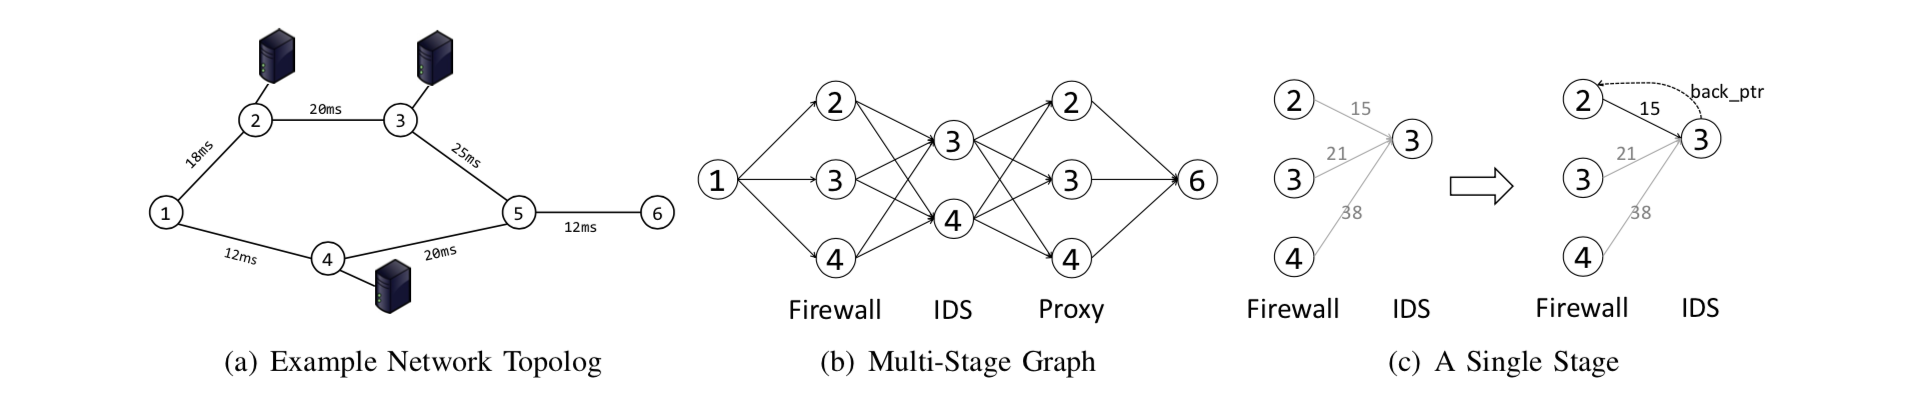
\includegraphics[width=\textwidth]{images/bari.png}
  \caption{\cite{Bari2015} algorithm transmissions to create multi-stage graph}
\end{figure}

\cite{AbuLebdeh2017} considers the VNF placement is know a prior so we must used its algorithm after the VNF placement.
Therefore, to comparing MASMAN with \cite{AbuLebdeh2017} as the nearest work to JSD-MP,
We use the Bari \cite{Bari2015} algorithm for the placement and then use the proposed way in the \cite{AbuLebdeh2017} for VNFM placement.
The proposed way in \cite{AbuLebdeh2017} use Tabu Search for finding the best VNFM placement.
The results of this comparasion are availabe at the following sections.

%% Complexity analysis


\section{Evaluation and Numerical Results}\label{sec:results}
\hly{
a) Simulation settings: Topologies and all other parameters used in simulation it is better to use a table \\
The algorithms which are simulated \\
Parameters used for evaluation \\
b) A subsection per parameter\\
Emphasize on achievements\\
}
\subsection{Joint vs Disjoint}\label{sec:joint-vs-disjoint}
Here we want to compare the joint and disjoint solutions.
For this comparison we use two different topology to have better insights and fair results.

\subsubsection{FatTree}
Here we will use FatTree topology with k equals to 6.
As you can see results confirm our hypothesis that joint solutions makes better revenues.

\begin{table}[H]
    \caption{Revenues from Joint and Disjoint Solutions on FatTree Topology with k equals to 6}
    \label{tbl:joint-vs-disjoin-fattree}
    \medskip
    \centering
    \begin{tabular}{lrrr}
        \toprule
        {} &    joint &  disjoint &  nchains \\
        \midrule
        0 &  45440.0 &   44980.0 &      100 \\
        1 &  36660.0 &   17090.0 &       80 \\
        2 &  27850.0 &   13340.0 &       60 \\
        3 &  18340.0 &   13440.0 &       40 \\
        4 &   9170.0 &    1880.0 &       20 \\
        \bottomrule
    \end{tabular}
\end{table}

\begin{figure}[H]
    \centering
    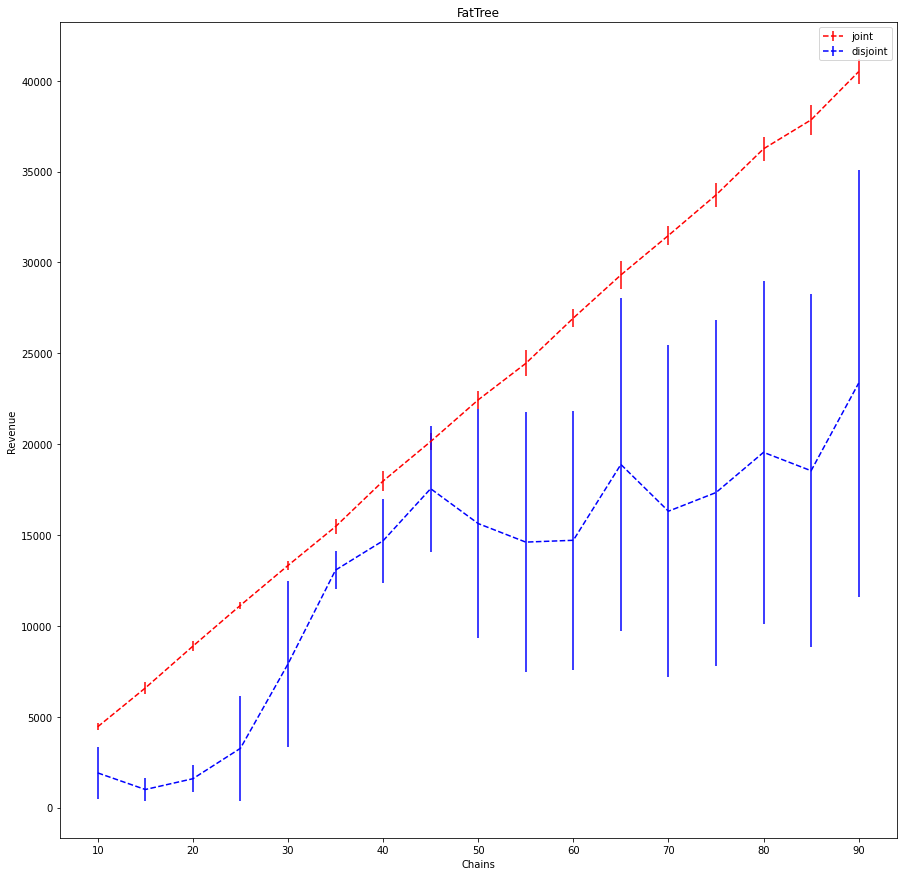
\includegraphics[height=350pt]{plots/joint-vs-disjoint-fattree.png}
    \caption{Revenues from Joint and Disjoint Solutions on FatTree Topology with k equals to 6}
    \label{fig:joint-vs-disjoint-fattree}
\end{figure}

\subsection{USNet}
Here we will use USNet topology with 3 to 4 nodes attached to each of its points.
As you can see the results show joint and disjoint solutions on this setup work equally because there is no specific
management requirement and topology can handle all chains.

\begin{table}[H]
    \caption{Revenues from Joint and Disjoint Solutions on USNet Topology}
    \label{tbl:joint-vs-disjoin-usnet}
    \medskip
    \centering
    \begin{tabular}{lrrr}
        \toprule
        {} &    joint &  disjoint &  nchains \\
        \midrule
        0 &  23000.0 &   23010.0 &       50 \\
        1 &  34180.0 &   34260.0 &       75 \\
        2 &  45430.0 &   45560.0 &      100 \\
        3 &  57180.0 &   57380.0 &      125 \\
        4 &  68750.0 &   69360.0 &      150 \\
        \bottomrule
    \end{tabular}
\end{table}

\begin{figure}[H]
    \centering
    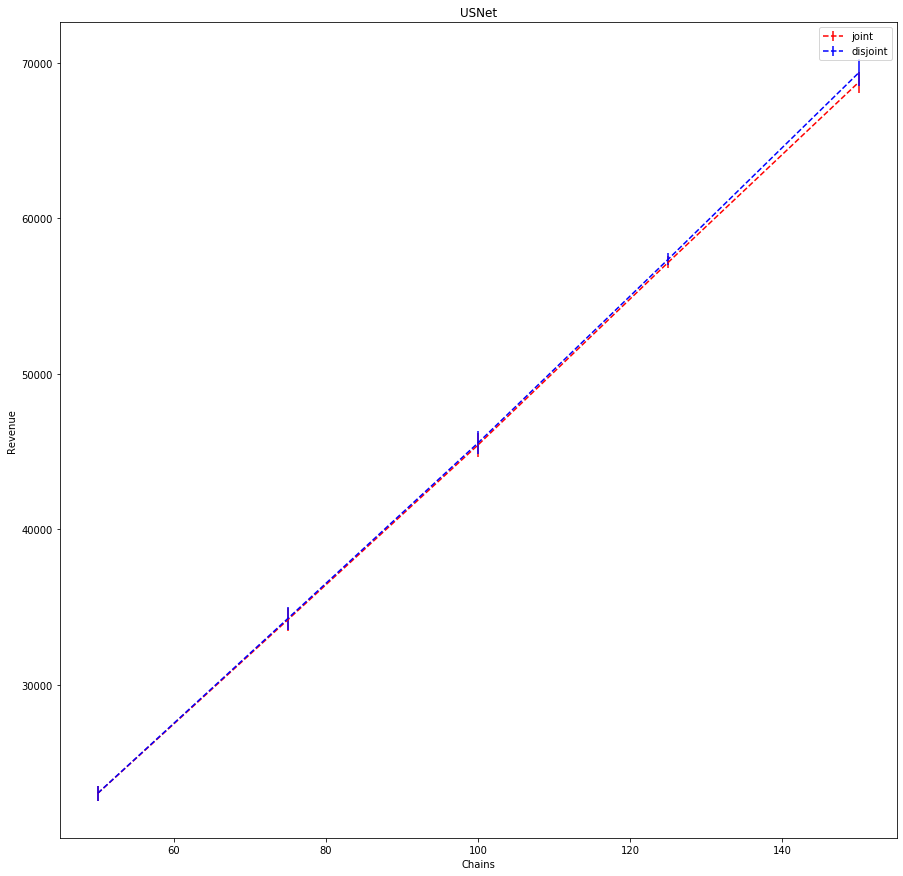
\includegraphics[height=350pt]{plots/joint-vs-disjoint-usnet.png}
    \caption{Revenues from Joint and Disjoint Solutions on USNet Topology}
    \label{fig:joint-vs-disjoint-usnet}
\end{figure}


\section{Conclusion and Future Work}\label{sec:conclusion}
\hly{
a) Review of what we have done \\
b) What is the future step \\
}

\bibliography{references}

\end{document}
